\chapter{\protect Introduction}
\label{introduction}

According to Hindu cosmological mythology, ancient people believe that a giant turtle bears the world on its back. Even after we stepped onto the moon at 1969, there are still plenty that we cannot explain. Recently, a group of scientists put a dilute NH$_4$CN in temperature of liquid nitrogen for 27 years and discovered an amino-acid : adenine \cite{miyakawa2002cold}. NH$_4^+$CN$^-$ plays an important role in life evolution. The formation of CN$^-$ is proposed by Kim and Kaiser (2001) \cite{kim},which comes from ammonia (NH$_3$) and methane (CH$_4$). However, they have only demonstrated the effects of cosmic rays (energetic electrons) onto the ice mixture, the photolysis experiments of CH$_4$+NH$_3$ ice mixtures are still not well understood. This thesis aimed to investigate the chemistry of VUV and EUV irradiations on CH$_4$+NH$_3$ ice mixtures, which is possibly one of the main starting components to form CN$^-$ in astrophysical environments.

NH$_3$ is often not found in astrophysical environments unless detecting aimbiguously. Nearly all the far-infra red bands expect region 2.2 $\mu$m overlapps with water. As one of the icy satellites, the New Horizons team have discovered a high concentration crater of NH$_3$(figure \ref{fig:Charon_IR} on Charon\cite{grundy2016surface}. Also, models of Hoey et al.(2017)\cite{hoey2017rarefied} used potential energy fields to simulate the amount of Pluto ejectas during New horizons' approach. Among which 98 \% of the arrived ejecta is CH$_4$ (figure \ref{fig:Charon_distribution}).


\begin{figure}
\centering
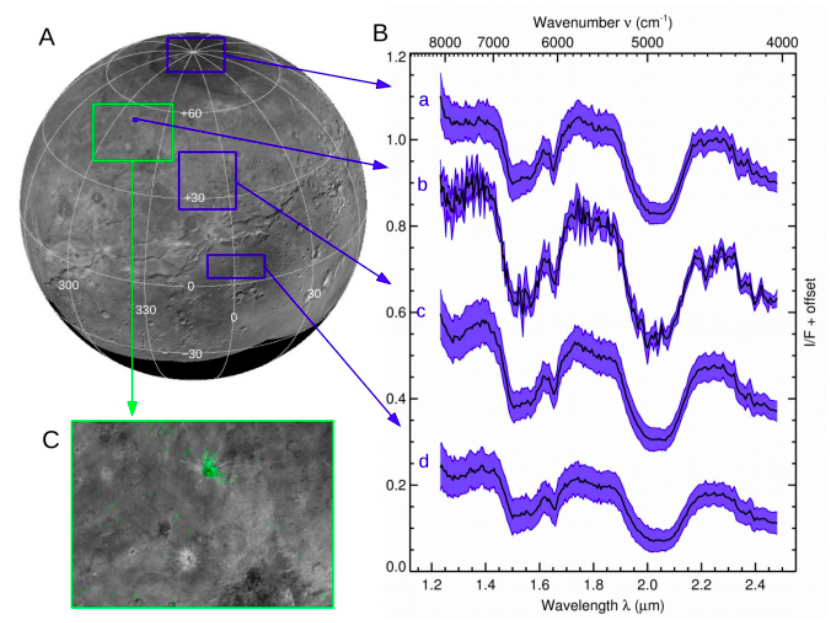
\includegraphics[width=\textwidth]{figures/chapter1/IR.png}
\caption{The 2.2$\mu$m absorption taken by LEISA camera colored as green on the topology shown by LORRI camera (A) and the spectra at 4 positions with b taken near organa crater.(quoted from \cite{grundy2016surface})}
\label{fig:Charon_IR}
\end{figure}

\begin{figure}
\centering
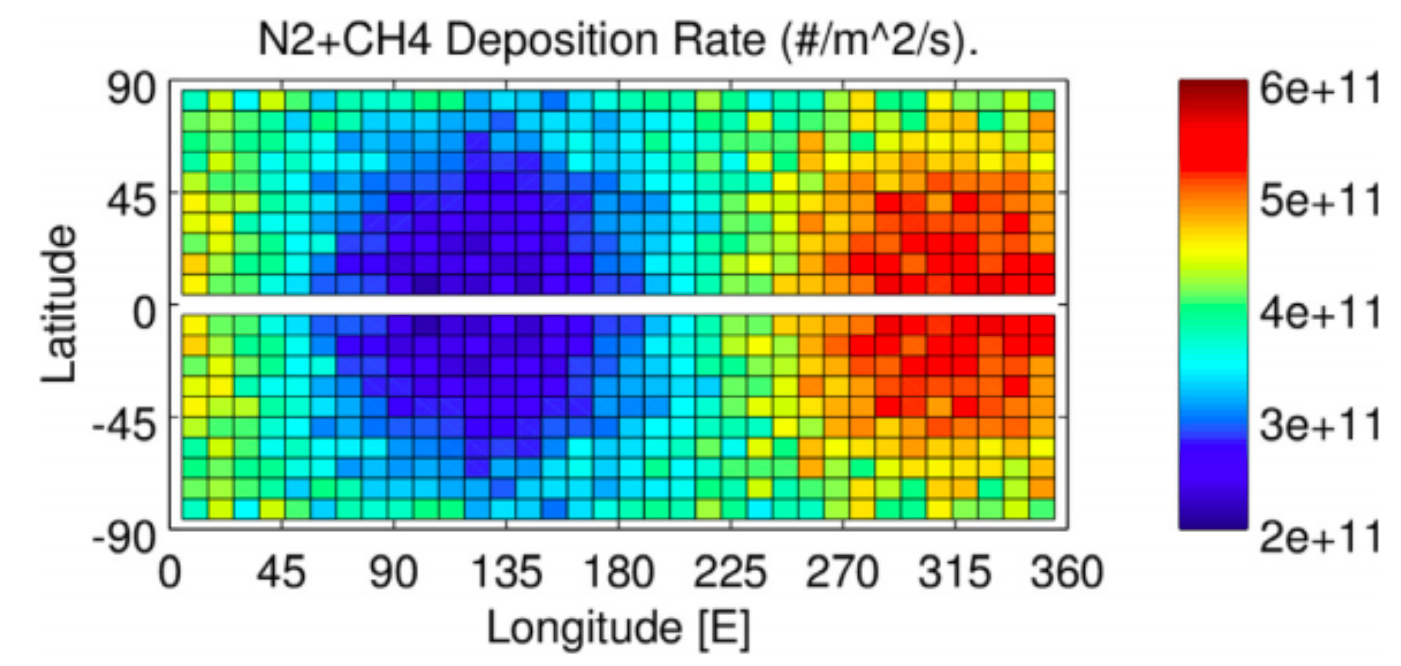
\includegraphics[width=\textwidth]{figures/chapter1/methane.png}
\caption{The simulation of N$_2$ and CH$_4$ model assuming all arrived molecules will stick onto the surface of Charon. Among the deposition rate, 98 \% of them are CH$_4$ because CH$_4$ is lighter and preferentially escapes. The molar fraction of CH$_4$ increase from hypothesized 0.44 \% to 42 \% in the exobase of Pluto.(quoted from \cite{hoey2017rarefied})}
\label{fig:Charon_distribution}
\end{figure}

With both methane and ammonia, we still need energy to generate CN$^-$. There exsists many energetic sources in our solar system, they include solar wind, irradiation from the sun, cosmic rays from the outer solar system, etc. Among these, Ly-$\alpha$ appears to be the largest source in the dark side of Charon. It is attributioned from both solar occultation (70 \%) and resonance scattering by atomic hydrogen flow (30 \%) in the solar system. Its flux is $3.5 \times 10^7$ photons cm$^{-2}$ s$^{-1}$ at the winter pole of Charon \cite{grundy2016formation} which is 50 \% larger than expected before Mission New Horizons \cite{gladstone2015lyalpha}. We performed VUV irradiation on CH$_4$+NH$_3$ experiments with different ratios (including 3:2, 1:5, 1:10 and 1:20) to simulate the effect of Ly-$\alpha$ on different concentrations of CH$_4$, which deposits at temperature below 25 K at pressure $7.4 \times 10^{-14}$ torr onto the surface of Charon. The time for depositing CH$_4$ is 2 times longer at the pole (130 earth years) than at 45$^{\circ}$ lattitude \cite{grundy2016formation} (figure \ref{fig:Charon_thermal}).

\begin{figure}
\centering
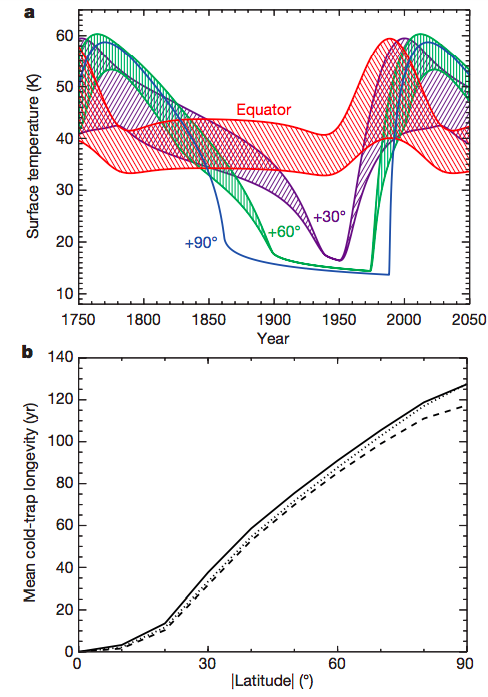
\includegraphics[width=0.5\textwidth]{figures/chapter1/thermal.png}
\caption{The temperature of Charon with thermal inertia 10 J m$^{-2}$ K$^{-1}$ s$^{-1/2}$ in 1750 to 2050 Earth years (a) and longest time the Latitude is under 25 K with the model averaged for 3 Myr with 2.5 (solid) 10 (dotted) and 40 (dashed) J m$^{-2}$ K$^{-1}$ s$^{-1/2}$ (b).(quoted from \cite{grundy2016formation})}
\label{fig:Charon_thermal}
\end{figure}

Apart from VUV irradiation, EUV irradiation also took part. The EUV irradiation (>12.4 eV) is $8.7 \times 10^7$ eV cm$^{-2}$ s$^{-1}$ at mean heliocentric distance 39 A.U. whereas VUV irradiation (Ly-$\alpha$) is $1.9 \times 10^9$ eV cm$^{-2}$ s$^{-1}$\cite{grundy2016formation}. In order to investigate the effectiveness of EUV to VUV irradiation, we kept temperature of CH$_4$+NH$_3$ (3:2 \& 1:5) ice mixtures at 15 K and use the monochromatic 30.4 nm (He II) light provided by High flux beamline at National Synchrotron Radiation Research Centre (NSRRC) in Taiwan to irradiate the ice mixtures.

In this text, we will introduce the experimental methodology in chapter \ref{methods}, theformation reaction mechanisms of CH$_4$+NH$_3$ ice mixtures in EUV and VUV irradiation, a brief relation of our residues with tholin on Titan will be made in chapter \ref{results}. With these results, we will have a better understanding about Charon, different energy sources including electron irradiation experiments , EUV and VUV irradiations, and their astrophysical implications will be presented in chapter \ref{astron}.
